\section{Durchführung}
\label{sec:Durchführung}

Im vorliegenden Experiment wird ein $\alpha$-Strahler verwendet, welcher sich, wie in Abbildung \ref{fig:aufbau} 
dargestellt, auf einer Schiene in einem Glaszylinder befindet. Mithilfe einer Vakuumpumpe kann diese
evakuiert werden. Der Druckunterschied zum Atmosphärendruck wird an einem Manometer abgelesen.
Über die Schiene kann der Abstand der Strahlungsquelle zum Detektor fest gewählt werden. Dieser 
Halbleiterdetektor ist in der Lage, sowohl die Anzahl der Impulse als auch die relative Energie 
der $\alpha$-Teilchen zu messen. Die grundlegende Funktionsweise ist, dass durch die Strahlung 
Elektron-Loch-Paare entstehen, sodass freie Ladungen entstehen. Diese werden an Elektroden 
registiert und der vom Vorverstärker verstärkte Puls kann verarbeitet werden. Im vorliegenden 
Versuchsaufbau wird diese Auswertung über das Computerprogramm Multichannel Analyzer realisiert. 
Dieses bietet unter anderem die Möglichkeit, die Gesamtzählrate über einen festgelegten Zeitraum 
sowie eine Pulshöhenanalyse durchzuführen. 

\begin{figure}
  \centering
  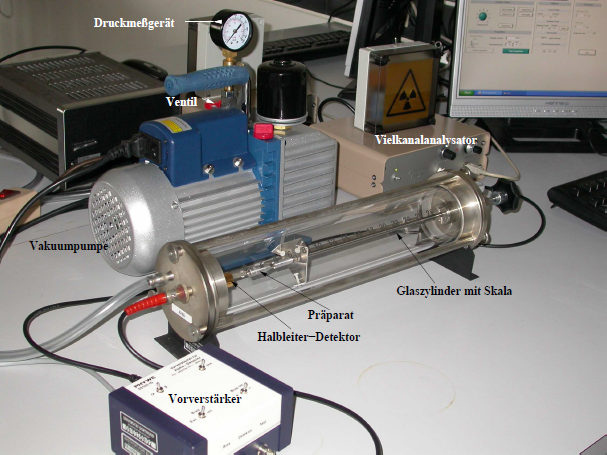
\includegraphics[scale=0.3]{content/Aufbau.png}
  \caption{Versuchsaufbau zur Bestimmung der Reichweite von $\alpha$-Strahlung. [1]}
  \label{fig:aufbau}
\end{figure}

Vor Beginn der eigentlichen Messung wird die Strahlungsquelle zunächst möglichst weit vom Sperrschichtzähler
entfernt und die Diskriminatorschwelle des Zählers auf den Grenzwert eingestellt, ab welchem bei Normaldruck 
keine Impulse mehr detektiert werden. Danach wird der Glaszylinder evakuiert und die radioaktive Probe so weit 
an den Detektor herangeschoben, bis dieser anfängt vereinzelte $\alpha$-Teilchen zu zählen. \\
Nun wird der Druck von $\SI{0}{\milli\bar}$ bis ca. $\SI{1000}{\milli\bar}$ Normaldruck in $\SI{50}{\milli\bar}$ 
Schritten erhöht und für jweils $\SI{120}{\second}$ eine Messung durchgeführt. Es werden vom Computerbildschirm für 
jeden Messabschnitt die Gesamtzählrate und der Messkanal mit der maximalen Zählrate abgelesen und notiert. \\
Anschließend wird die Strahlungsquelle um $\SI{0.5}{\centi\meter}$ weg vom Sperrschichtzähler entfernt und die 
gleiche Messung erneut durchgeführt. \\
Im letzten Schritt wird bei unveränderten Abstand und einem evakuierten Glaszylinder 100 mal die Gesamtzählrate 
in einem Zeitraum von $\SI{10}{\second}$ gemessen. 